\chapter{Modélisation du système}
\label{chapitre.modele}
\section{Choix du modèle et conséquences}
	\subsection{Objectifs}
		L'objectif de ce chapitre est de présenter une modélisation dynamique d'un robot humanoïde possédant une base mobile à roues omnidirectionnelles. 
		Ce modèle doit apporter un bon compromis entre fidélité vis à vis du comportement du robot réel et complexité, qui impacte de manière directe le temps de calcul.
		Notamment, on montre qu'il n'est pas nécessaire de modéliser tout les paramètres du robot : représenter uniquement les dynamiques principales suffit à obtenir un contrôle précis du robot. 
		La section \ref{section.closedloop} détaillera les méthodes de compensation des éléments non modélisés.
	
		\fig{
			\centering
			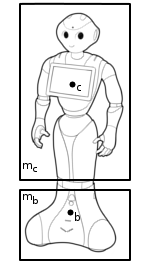
\includegraphics[width=2in]{modele.png}
			\caption{Représentation globale du modèle dynamique.}
			\label{fig.modele}
		}
		
	\subsection{Avantages du modèle}
		
		Le choix se porte sur une modélisation dynamique d'un robot rigide multi-corps. 
		Le modèle présenté \rfi{fig.modele} comporte deux corps. Le premier est attaché à la base mobile, de masse $m_b$ et de position du centre de masse (CoM) $\bar{b}$.
		Le second modélise le corps du robot, de masse $m_c$ et de CoM $\bar{c}$.
		
		Le choix d'un modèle à deux corps permet de prendre en compte la rotation générale du corps du robot autour de la base mobile.
		Cette modélisation est pertinente dans le cas où les bras du robot ne génèrent que peu ou pas de moment angulaire.
		Dans le cas contraire, nous considérerons que les effets parasites dûs aux mouvements des bras pourront être compensés correctement par le schéma de contrôle en boucle fermée présenté en section \ref{section.closedloop}.
		Le choix de ce modèle est également conditionné par la répartition massique de la plate-forme expérimentale :
		Elle est principalement concentré en deux zones, qui correspondent aux corps choisis : la base mobile et le torse du robot.	
	
	\subsection{Inconvénients du modèle}
		
		Le choix d'un modèle rigide multi-corps implique que les éléments suivants ne seront pas modélisés :
		\liste{
			\item 	Les différentes élasticités. Les technologies d'actionnement utilisées sur la plate-forme expérimentale ne comportent pas d'élasticités notables.
				Le seul élément compliant est un ensemble de deux bandes élastiques attachées à l'articulation du roulis de la hanche permettant au robot de maintenir une posture droite en l'absence de contrôle du moteur.
				Cet élément est négligeable en terme de dynamique car la raideur associée est très faible.
			\item	Les jeux mécaniques présents sur le robot. Ceux-ci sont présents sur la plate-forme expérimentale, du fait des systèmes de réduction entre les moteurs et les articulations basés sur des engrenages.
				Les effets dynamiques parasites apportés par le jeu mécanique ne sont pas négligeables.
				Cependant, il peuvent être compensés de manière suffisamment efficace (plus de détails en section \ref{section.closedloop}) pour que cela soit transparent du point de vue de la commande présentée dans le chapitre \ref{chapitre.commande}.
			\item	Les glissements pouvant survenir entre les roues du robot et le sols ne sont pas modélisés. 
				Ceux-ci peuvent être néanmoins handicapants, car le système devient en partie non-observable en présence de glissement (plus de détails en section \ref{section.observateurbase}).
				Une solution a été apportée en section \ref{section.objectifs3roues} afin de limiter leurs possibilités d'apparition ainsi que leurs impacts sur la dynamique du robot.
			\item	Le nombre de corps choisi pour cette modélisation dynamique est nécessairement plus faible que le nombre de corps réels présents sur le robot, pour des raisons de complexité du modèle.
				Ainsi, tout les effets dynamiques ne pourront pas être représentés. Le choix du nombre de corps, et de leurs propriétés doit permettre de rendre négligeable les dynamiques non modélisées.
				Le développement d'une solution optimale du choix du nombre de corps et de leurs propriétés est présenté en annexe \ref{annexe.choixmodele}.
		}
		

	\section{Modélisation dynamique}
	\label{section.modelisation_dynamique}

		\subsection{Problème de complémentarité mixte}
		
			\subsubsection{Géométrie du robot}
			\label{section.geometrie}
		
				On considère le robot modélisé par deux corps $\bar{b}$ et $\bar{c}$ de masse associée $m_b$ et $m_c$. 
				Ces corps sont en contact avec le sol par l'intermédiaire de trois points $p_f$, $p_r$ et $p_l$ correspondant aux trois points de contact des roues avec le sol \rfi{fig.bascule}.
				La roue avant gauche correspond au point $p_r$, la roue avant droite au point $p_l$ et la roue arrière au point $p_f$.
				(On associe l'indice $r$, $f$ et $l$ au sens du basculement, la roue en l'air lors de ce basculement correspond. Pour un basculement vers la droite, la roue en l'air correspond à la roue avant gauche.)
				
				
				On considère que le système peut se retrouver dans quatre modes dynamiques différents :
				\liste{
					\item Le robot ne bascule pas et les trois roues sont en contact avec le sol.
					\item Le robot est en rotation vers l'avant autour de l'axe défini par les deux roues avant. On note l'angle de rotation $\psi_f$. La roue arrière est dans ce cas en l'air.
					\item Le robot est en rotation vers la gauche autour de l'axe défini par la roue avant gauche et la roue arrière. On note l'angle de rotation $\psi_l$. La roue avant droite est dans ce cas en l'air.
					\item Le robot est en rotation vers la droite autour de l'axe défini par la roue avant droite et la roue arrière. On note l'angle de rotation $\psi_r$. La roue avant gauche est dans ce cas en l'air.
				}
				Enfin, on considère la répartition de la masse de chaque corps concentrée en un seul point, son CoM. Ainsi, il n'y a aucune inertie de rotation associée à $\bar{b}$ ou $\bar{c}$.
				
				\fig{
					\centering
					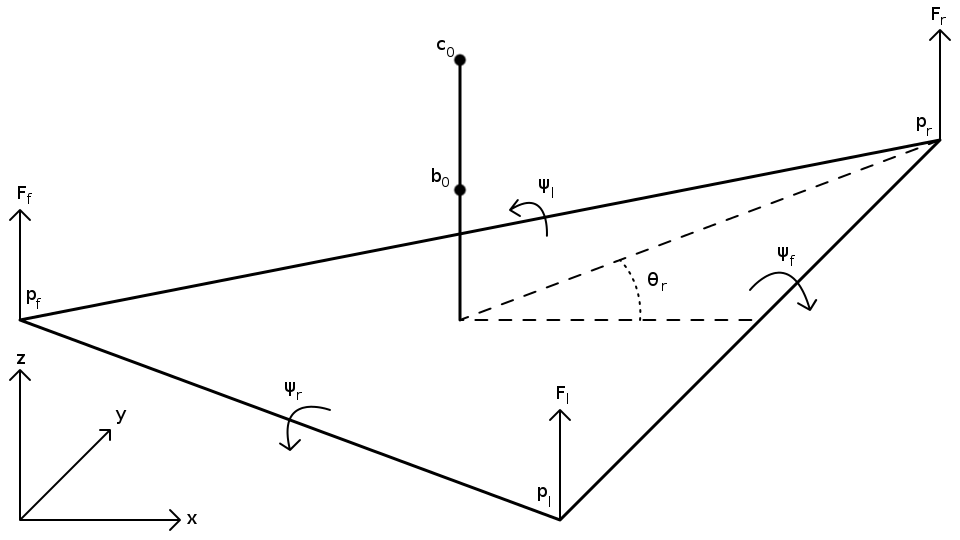
\includegraphics[width=6.5in]{bascule.png}
					\caption{représentation dans le repère $\rep_w$ des points de contacts avec le sol et des angles de basculement.}
					\label{fig.bascule}
				}
				
			\subsubsection{Hypothèses}
			\label{section.hypothese}
			
				Dans la suite, nous considèrerons un repère galiléen fixe orthonormé direct $\rep_w(O, \vec{x},\vec{y},\vec{z})$, $\vec{x}$ étant orienté vers l'avant du robot, $\vec{y}$ vers la gauche, et $\vec{z}$ vers le haut. 
				Ce repère est attaché au sol, $\vec{x}$ et $\vec{y}$ inclus dans le plan du sol, et $\vec{z}$ orthogonal au sol. 
				Celui-ci n'est pas forcément horizontal, ce qui implique que le vecteur gravité ne soit pas forcément orienté selon l'axe $\vec{z}$.
					
				Nous allons définir deux hypothèses conditionnant de façon importante la modélisation du système :
				\liste{
					\item 	Comme il a été défini en section \rf{section.geometrie}, nous considérons que le robot ne peut se retrouver que sur trois ou deux roues en contact avec le sol.
						Cela implique que nous ne traitons pas les cas où le robot bascule sur une roue ou est en chute libre.
					\item	La masse du robot étant principalement concentrée sur son axe de rotation selon $\vec{z}$, nous pouvons négliger les effets dynamiques induits par la rotation du robot.
					        Nous considérons donc l'angle de rotation du robot autour de l'axe $\vec{z}$ comme constant.
				}
			
			\subsubsection{Cinématique directe}
			
				\subsubsubsection{Notations}
					
					Premièrement, nous considérons que la position des corps $\bar{c}$ et $\bar{b}$ est obtenue par la composition de trois éléments :
					\liste{
						\item $r$, la position générale du centre géométrique de la base mobile projeté sur le sol et exprimée dans le repère $\rep_w$.
						\item $\delta_c$ et $\delta_b$, les longueurs apportées par l'actionnement des moteurs.
						\item $\psi_f$, $\psi_r$ et $\psi_l$, les rotations apportées par le basculement du robot sur chacun de ses cotés.
					}
					
					Afin de pouvoir écrire les équations cinématiques, nous avons besoin de définir différentes grandeurs dépendantes de la géométrie du robot. 

					
					$\forall i\in\{f,r,l\}$ :
					
					On note $\theta_i$ l'angle dans le plan $(\vec{x}, \vec{y})$ que fait la droite reliant le centre de la base mobile et la roue $i$ avec l'axe $\vec{x}$ \rfi{fig.bascule}:
					\eq{
						\cos(\theta_i)= \overrightarrow{rp_i} \cdot \vec{x}
					}
					
						
					On note  $\vec{n_i}$ l'axe défini par la droite reliant le centre de la base mobile $r$ et la roue $i$, et $\vec{t_i}$ son axe orthogonal inclus dans le plan $(\vec{x}, \vec{y})$ :
					\eqa{
						\vec{n_i} &= \frac{\overrightarrow{r^{xy}~p_i^{xy}}}{\norm{\overrightarrow{r^{xy}~p_i^{xy}}}} \\
						\vec{t_i} &= \vec{z} \times \vec{n_i}
					}
					$\rep_i$ représente le repère $(O, \vec{n}_i, \vec{t}_i, \vec{z})$.
					
					On note $D_i$ la distance entre la position $p_i$ de la roue $i$ et la position de la projection des deux autres roues sur l'axe $\vec{n_i}$ 
					(les deux points projetés sont confondus sur l'axe $\vec{n_i}$ car le triangle formé par la base mobile est équilatéral) \rfi{fig.lagrange}:
					\eq{
					  D_i = \norm{p_i - p_j \cdot \vec{n_i}}
					}
					avec $j\in\{f,r,l\} \neq i$.
					
					On note $d_i$ la distance dans le plan $(\vec{x}, \vec{y})$ entre le centre de la base mobile $r$ et la projection des deux autres roues sur l'axe $\vec{n_i}$ \rfi{fig.lagrange}:
					\eq{
						d_i = D_i - \norm{\overrightarrow{r^{xy}~p_i^{xy}}}
					}
					
					
					On note $h_b$ et $h_c$ les hauteurs initiales de $\bar{b}$ et $\bar{c}$ (lorsque $\delta_c=\delta_b=0$ et $\psi_f=\psi_r=\psi_l=0$) \rfi{fig.lagrange}.
					On introduit $c_0$ et $b_0$ les positions des corps $\bar{b}$ et $\bar{c}$ à leurs positions initiales \rfi{fig.bascule}:
					\eqa{
					\label{eq.c0}
						c_0 &= r+h_c\vec{z} \\
					\label{eq.b0}
						b_0 &= r+h_b\vec{z}
					}
					
					On note $l_{b_i}$ et $l_{c_i}$ les distances entre la position $p_i$ de la roue $i$ et les corps $\bar{b}$ et $\bar{c}$ à leurs positions initiales \rfi{fig.lagrange}:
					\eqa{
						l_{b_i} &= \norm{\overrightarrow{b_0p_i}} \\
						l_{c_i} &= \norm{\overrightarrow{c_0p_i}}
					}
					
					On note $\phi_{i_b}$ et $\phi_{i_c}$ les angles que font l'axe $\vec{z}$ avec les droites reliant les positions initiales des corps $b_0$, $c_0$ et la position $p_i$ de la roue $i$ \rfi{fig.lagrange}:
					\eqa{
						\cos(\phi_{i_b}) &= -\overrightarrow{p_ib_0} \cdot \vec{z} \\
						\cos(\phi_{i_c}) &= -\overrightarrow{p_ic_0} \cdot \vec{z}
					}
					
					Enfin, on introduit $b$ et $c$ les positions commandées des corps $\bar{b}$ et $\bar{c}$ \rfi{fig.lagrange}:
					\eqa{
					\label{eq.b}
						b &= b_0 \\
					\label{eq.c}
						c &= c_0+\delta_c
					}
					
					\fig{
						\centering
						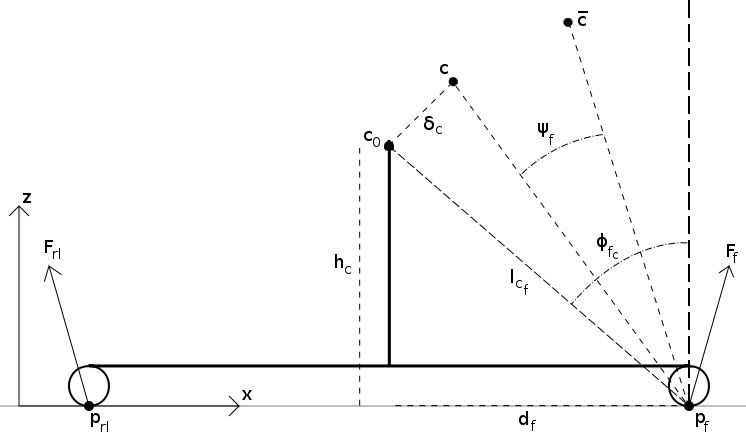
\includegraphics[width=6.5in]{lagrange.png}
						\caption{Projection dans le plan $(O,\vec{x}, \vec{z})$ du modèle du robot. 
							 Représentation des variables relatives au corps $\bar{c}$ et à l'angle $\psi_f$. 
							 Celles relatives à $\bar{b}$, $\psi_r$ et $\psi_l$ ne sont pas représentées, mais correspondent au même schéma.}
						\label{fig.lagrange}
					}
					
				\subsubsubsection{Equations cinématiques}
					
					Nous pouvons à présent écrire les équations cinématiques des points de contact des roues $p_f$, $p_r$ et $p_l$ \rfi{fig.lagrange}.
					$\forall i\in\{f,r,l\}$ :
					la position du point de contact $p_i$ peut s'exprimer comme la rotation d'angle $\psi_i$ et de rayon $D_i$ autour de l'axe défini par les deux autres roues, 
					puis déplacé par translation de la distance entre cet axe et la position de la base mobile $b$.
					\eq{
					\label{eq.p}
						\lst{
							p^x_i = b^x+\prt{d_i-D_i\cos(\psi_i)}\cos(\theta_{i}) \\
							p^y_i = b^y+\prt{d_i-D_i\cos(\psi_i)}\sin(\theta_{i}) \\
							p^z_i = b^z-h_b+D_i\sin(\psi_i)
						}
					}
					
					On peut écrire les équations cinématiques des corps $\bar{b}$ et $\bar{c}$ en sommant leurs positions initiales ($b_0$ et $c_0$) avec les longueurs d'actionnement ($\delta_c$ et $\delta_b$) et la contribution des basculements ($\psi_f$, $\psi_r$ et $\psi_l$).
					Cette somme n'est valable que si un seul des angles $\psi_f$, $\psi_r$ ou $\psi_l$ peut être non-nul à la fois, ce qui correspond aux hypothèses formulées en section \rf{section.hypothese}. 
					
					On écrit donc, concernant le corps $\bar{c}$ :
					\eq{
						\lst{
							\bar{c}^x = c_0^x+\delta^x+\dsomme{i\in\{f,r,l\}}{}{\prt{d_i+l_{c_i}\sin(\psi_i-\phi_{i_c})}\cos(\theta_{i})} \\
							\bar{c}^y = c_0^y+\delta^y+\dsomme{i\in\{f,r,l\}}{}{\prt{d_i+l_{c_i}\sin(\psi_i-\phi_{i_c})}\sin(\theta_{i})} \\
							\bar{c}^z = c_0^z+\delta^z+\dsomme{i\in\{f,r,l\}}{}{-h_c+l_{c_i}\cos(\psi_i-\phi_{i_c})}
						}
					}
					que l'on peut reformuler en utilisant l'équation \rf{eq.c} :
					\eq{
					\label{eq.bar_c}
						\lst{
							\bar{c}^x = c^x+\dsomme{i\in\{f,r,l\}}{}{\prt{d_i+l_{c_i}\sin(\psi_i-\phi_{i_c})}\cos(\theta_{i})} \\
							\bar{c}^y = c^y+\dsomme{i\in\{f,r,l\}}{}{\prt{d_i+l_{c_i}\sin(\psi_i-\phi_{i_c})}\sin(\theta_{i})} \\
							\bar{c}^z = c^z+\dsomme{i\in\{f,r,l\}}{}{-h_c+l_{c_i}\cos(\psi_i-\phi_{i_c})}
						}
					}
					et concernant le corps $\bar{b}$ :
					\eq{
					\label{eq.bar_b}
						\lst{
							\bar{b}^x = b^x+\dsomme{i\in\{f,r,l\}}{}{\prt{d_i+l_{b_i}\sin(\psi_i-\phi_{i_b})}\cos(\theta_{i})} \\
							\bar{b}^y = b^y+\dsomme{i\in\{f,r,l\}}{}{\prt{d_i+l_{b_i}\sin(\psi_i-\phi_{i_b})}\sin(\theta_{i})} \\
							\bar{b}^z = b^z+\dsomme{i\in\{f,r,l\}}{}{-h_b+l_{b_i}\cos(\psi_i-\phi_{i_b})}
						}
					}
					
				\subsubsubsection{Hypothèse d'angles de basculements faibles}
				
					Dans la suite, afin de simplifier les formulations des équations de la dynamique, nous allons établir dès maintenant une hypothèse : Les angles $\psi_{frb}$ sont considérés proches de $0$.
					Dans le cas où le robot ne bascule pas, cela est exact. Dans le cas où le robot bascule, on suppose que l'angle de basculement reste faible.
					Nous pouvons donc réécrire la formulation des équations cinétiques des corps $\bar{c}$ et $\bar{b}$ en utilisant une approximation au premier ordre autour de $\psi_f=\psi_r=\psi_l=0$ :
					\eqa{
						\bar{c}^x &= \initcond{\bar{c}^x}{\psi_{frl}=0} + \somme{i\in\{f,r,l\}}{}{\partiald{\bar{c}^x}{\psi_i}{\psi_{frl}=0} \psi_i} + o(\psi_{frl}^2) \\
						\bar{b}^x &= \initcond{\bar{b}^x}{\psi_{frl}=0} + \somme{i\in\{f,r,l\}}{}{\partiald{\bar{b}^x}{\psi_i}{\psi_{frl}=0} \psi_i} + o(\psi_{frl}^2)
					}
					
					Concernant le corps $\bar{c}$, l'équation \rf{eq.bar_c} s'approxime à l'ordre 1 par :
					\eq{
						\lst{
							\bar{c}^x \simeq c^x+\dsomme{i\in\{f,r,l\}}{}{\prt{d_i+l_{c_i}\sin(-\phi_{i_c})+\psi_il_{c_i}\cos(-\phi_{i_c})}\cos(\theta_{i})} \\
							\bar{c}^y \simeq c^y+\dsomme{i\in\{f,r,l\}}{}{\prt{d_i+l_{c_i}\sin(-\phi_{i_c})+\psi_il_{c_i}\cos(-\phi_{i_c})}\sin(\theta_{i})} \\
							\bar{c}^z \simeq c^z+\dsomme{i\in\{f,r,l\}}{}{-h_c+l_{c_i}\cos(-\phi_{i_c})-\psi_il_{c_i}\sin(-\phi_{i_c})}
						}
					}
					que l'on peut simplifier en relevant \rfi{fig.lagrange} que ($l_{c_i}\sin(\phi_{i_c}) = d_i$) et ($l_{c_i}\cos(\phi_{i_c}) = h_c$) :
					\eq{
					\label{eq.bar_c_appr}
						\lst{
							\bar{c}^x \simeq c^x+\dsomme{i\in\{f,r,l\}}{}{\psi_ih_c\cos(\theta_{i})} \\
							\bar{c}^y \simeq c^y+\dsomme{i\in\{f,r,l\}}{}{\psi_ih_c\sin(\theta_{i})} \\
							\bar{c}^z \simeq c^z+\dsomme{i\in\{f,r,l\}}{}{\psi_id_i}
						}
					}
					et de même concernant le corps $\bar{b}$ :
					\eq{
					\label{eq.bar_b_appr}
						\lst{
							\bar{b}^x \simeq b^x+\dsomme{i\in\{f,r,l\}}{}{\psi_ih_b\cos(\theta_{i})} \\
							\bar{b}^y \simeq b^y+\dsomme{i\in\{f,r,l\}}{}{\psi_ih_b\sin(\theta_{i})} \\
							\bar{b}^z \simeq b^z+\dsomme{i\in\{f,r,l\}}{}{\psi_id_i}
						}
					}
					
					Nous aurons également besoin dans la suite des équations approximées des positions des points de contact des roues avec le sol :
					\eq{
					\label{eq.p_appr}
						\lst{
							p^x_i \simeq b^x+(d_i-D_i)\cos(\theta_{i}) \\
							p^y_i \simeq b^y+(d_i-D_i)\sin(\theta_{i}) \\
							p^z_i \simeq b^z-h_b+D_i\psi_i
						}
					}

			
			\subsubsection{Énergies cinétiques et potentielles}
			
				\subsubsubsection{Contraintes sur le basculement du robot}
				\label{section.contrainte_basculement}
				
					Afin d'exprimer les équations du mouvement du robot, nous allons utiliser la méthode Lagrangienne.
					Celle-ci est pertinente dans notre cas car elle est particulièrement adaptée à la formulation sans ambiguïtés de systèmes dynamiques soumis à des forces de contraintes, comme les forces de réactions dues au sol sur les roues. 
					Pour cela, il nous faut dans un premier temps écrire les équations des énergies cinétiques $T$ et potentielles $V$ du système :
					
					\eqa{
						T &= \frac{1}{2}m_b(\dot{\bar{b}}^{x^2} + \dot{\bar{b}}^{y^2} + \dot{\bar{b}}^{z^2}) + \frac{1}{2}m_c(\dot{\bar{c}}^{x^2} + \dot{\bar{c}}^{y^2} + \dot{\bar{c}}^{z^2}) \\
						V &= m_bg^x\bar{b}^x + m_cg^x\bar{c}^x + m_bg^y\bar{b}^y + m_cg^y\bar{c}^y + m_bg^z\bar{b}^z + m_cg^z\bar{c}^z 
					}
					avec $g$ le vecteur gravité. On rappelle que le repère $\rep_w$ étant attaché au sol, le vecteur gravité n'est pas forcément orienté selon la direction verticale $\vec{z}$, car le sol peut ne pas être horizontal.
					
					De plus, l'angle de rotation du robot autour de l'axe $\vec{z}$ étant considéré comme constant, il n'intervient pas dans l'expression de l’énergie cinétique $T$. 
					
					Un seul des angles $\psi_f$, $\psi_r$ ou $\psi_l$ peut être non-nul à la fois. Cela s'exprime par la contrainte suivante :
					\eq{
						\label{eq.contrainte_psi_ij}
						\forall (i,j)\in\{f, r, l\},~ i\neq j,~~ \psi_i\psi_j=0
					}
					
				\subsubsubsection{Formulation des énergies cinétiques et potentielles}
				
					En dérivant les équations cinématiques \rf{eq.bar_c_appr}\rf{eq.bar_b_appr} et en utilisant la contrainte précédente \rf{eq.contrainte_psi_ij}, nous pouvons exprimer les vitesses des corps $\bar{c}$ et $\bar{b}$ élevées au carré.
					\eqa{
						\dot{\bar{c}}^{x^2} &= \dot{c}^{x^2} + h_c^2\somme{i\in\{f, r, l\}}{}{\cos(\theta_i)^2\dot{\psi}_i^2} + 2h_c\dot{c}^x\somme{i\in\{f, r, l\}}{}{\cos(\theta_i)\dot{\psi}_i} \\
						\dot{\bar{c}}^{y^2} &= \dot{c}^{y^2} + h_c^2\somme{i\in\{f, r, l\}}{}{\sin(\theta_i)^2\dot{\psi}_i^2} + 2h_c\dot{c}^y\somme{i\in\{f, r, l\}}{}{\sin(\theta_i)\dot{\psi}_i}\\
						\dot{\bar{c}}^{z^2} &= \dot{c}^{z^2} + \somme{i\in\{f, r, l\}}{}{d_i^2\dot{\psi}_i^2} + 2\dot{c}^{z}\somme{i\in\{f, r, l\}}{}{d_i\dot{\psi}_i} \\
						\dot{\bar{b}}^{x^2} &= \dot{b}^{x^2} + h_b^2\somme{i\in\{f, r, l\}}{}{\cos(\theta_i)^2\dot{\psi}_i^2} + 2h_b\dot{b}^x\somme{i\in\{f, r, l\}}{}{\cos(\theta_i)\dot{\psi}_i} \\
						\dot{\bar{b}}^{y^2} &= \dot{b}^{y^2} + h_b^2\somme{i\in\{f, r, l\}}{}{\sin(\theta_i)^2\dot{\psi}_i^2} + 2h_b\dot{b}^y\somme{i\in\{f, r, l\}}{}{\sin(\theta_i)\dot{\psi}_i}\\
						\dot{\bar{b}}^{z^2} &= \dot{b}^{z^2} + \somme{i\in\{f, r, l\}}{}{d_i^2\dot{\psi}_i^2} + 2\dot{b}^{z}\somme{i\in\{f, r, l\}}{}{d_i\dot{\psi}_i}
					}
			
				
					Nous obtenons donc la formulation des énergies cinétiques et potentielles en fonction des variables du système :
					
					\eqa{
						\nonumber T &= \frac{1}{2}m_b(\dot{b}^{x^2}+\dot{b}^{y^2}+\dot{b}^{z^2}) + \frac{1}{2}m_c(\dot{c}^{x^2}+\dot{c}^{y^2}+\dot{c}^{z^2}) + \frac{1}{2}(m_bh_b^2+m_ch_c^2)\somme{i\in\{f, r, l\}}{}{\dot{\psi}_i^2}\\
						\nonumber  &+ \frac{1}{2}(m_c+m_b)\somme{i\in\{f, r, l\}}{}{d_i^2\dot{\psi}_i^2}  + (m_ch_c\dot{c}^z+m_bh_b\dot{b}^z)\somme{i\in\{f, r, l\}}{}{d_i\dot{\psi}_i} \\
					\label{eq.T}
						&+ (m_bh_b\dot{b}^x+m_ch_c\dot{c}^x)\somme{i\in\{f, r, l\}}{}{\cos(\theta_i)\dot{\psi}_i} + (m_bh_b\dot{b}^y+m_ch_c\dot{c}^y)\somme{i\in\{f, r, l\}}{}{\sin(\theta_i)\dot{\psi}_i}
					}
					\eqa{
						\nonumber V &= m_bg^xb^x + m_cg^xc^x + m_bg^yb^y + m_cg^yc^y + m_bg^zb^z + m_cg^zc^z \\
						\nonumber &+ (m_bg^x h_b + m_cg^x h_c)\somme{i\in\{f, r, l\}}{}{\cos(\theta_i)\psi_i} + (m_bg^y h_b + m_cg^y h_c)\somme{i\in\{f, r, l\}}{}{\sin(\theta_i)\psi_i} \\
					\label{eq.V}
						&+(m_b+m_c)g^z\somme{i\in\{f, r, l\}}{}{d_i\psi_i}
					}			
					
			
			\subsubsection{Coordonnées généralisées et Lagrangien}
			
				L'étape suivante de la méthode Lagrangienne consiste à exprimer l'équation du Lagrangien en fonction des coordonnées généralisées choisies.
				
				Habituellement, le choix des coordonnées généralisées correspondent aux degrés de libertés du système. 
				Afin de faciliter la formulation du modèle, nous allons plutôt utiliser le jeu de coordonnées $q$ suivant, qui possède plus de variables que les degrés de libertés du système :
				\eq{
					q = \tr{\mat{b^x & b^y & b^z & c^x & c^y & c^z & \psi_f & \psi_r & \psi_l} }
				}
								
				Le choix d'utiliser les trois angles $\psi_{frl}$ pour représenter la rotation du système autour des trois directions possible permettra par la suite d'exprimer plus simplement les équations de la dynamique.
				
				
				Le Lagrangien $L$ du système est exprimé à partir des énergies cinétiques et potentielles de la façon suivante :
				\eq{
					L = T - V
				}
				
			\subsubsection{Application du principe de moindre action}	
			
				\subsubsubsection{Définitions}
				
					On défini l'action du système comme l'intégrale temporelle du Lagrangien. 
					Le principe de moindre action énonce que, dans le cas d'un système Lagrangien, l'action est stationnaire.
					Lorsque celui-ci est contraint par des forces de contact, le principe de moindre action permet d'écrire :
					\eq{
					\label{eq.lagrange}
						\forall{q_i\in q},~~~~\frac{d}{dt}\frac{\partial L}{\partial \dot{q}_i} - \frac{\partial L}{\partial q_i} = \somme{j\in\{f,r,l\}}{k\in\{x,y,z\}}{\dfrac{\partial p_{j}^k}{\partial q_i}F_{p_{j}}^k}
					}
					
					Afin de clarifier l'écriture des équations de la dynamique, on pose :
					\eqa{
						m_{hc} &= m_ch_c \\
						m_{hb} &= m_bh_b \\
						m_{q} &= m_{hc}h_c+m_{hb}h_b \\
						m_t &= m_c+m_b \\
						C_{\theta_i} &= \cos(\theta_i) \\
						S_{\theta_i} &= \sin(\theta_i)
					}
				
				\subsubsubsection{Équations de la dynamique}
				
					Les éléments de l'équation \rf{eq.lagrange} peuvent être calculés à l'aide des équations des énergies \rf{eq.T}\rf{eq.V} ainsi que des équations cinématiques \rf{eq.p} :
					\eqa{
						\label{eq.T_lagrange}
						\frac{d}{dt}\frac{\partial L}{\partial \dot{q}} &=
						\mat{
							m_b\ddot{b}^x+m_bh_b\somme{i\in\{f, r, l\}}{}{C_{\theta_i}\ddot{\psi}_i} \\
							m_b\ddot{b}^y+m_bh_b\somme{i\in\{f, r, l\}}{}{S_{\theta_i}\ddot{\psi}_i} \\
							m_b\ddot{b}^z+m_bh_b\somme{i\in\{f, r, l\}}{}{d_i\ddot{\psi}_i} \\
							m_c\ddot{c}^x+m_ch_c\somme{i\in\{f, r, l\}}{}{C_{\theta_i}\ddot{\psi}_i} \\
							m_c\ddot{c}^y+m_ch_c\somme{i\in\{f, r, l\}}{}{S_{\theta_i}\ddot{\psi}_i} \\
							m_c\ddot{c}^z+m_ch_c\somme{i\in\{f, r, l\}}{}{d_i\ddot{\psi}_i} \\
							(m_q + m_td^2_f)\ddot{\psi}_f + m_{hb}(C_{\theta_f}\ddot{b}^x+S_{\theta_f}\ddot{b}^y-d_f\ddot{b}^z) + m_{hc}(C_{\theta_f}\ddot{c}^x+S_{\theta_f}\ddot{c}^y+d_f\ddot{c}^z) \\
							(m_q + m_td^2_r)\ddot{\psi}_r + m_{hb}(C_{\theta_r}\ddot{b}^x+S_{\theta_r}\ddot{b}^y-d_r\ddot{b}^z) + m_{hc}(C_{\theta_r}\ddot{c}^x+S_{\theta_r}\ddot{c}^y+d_r\ddot{c}^z) \\
							(m_q + m_td^2_l)\ddot{\psi}_l + m_{hb}(C_{\theta_l}\ddot{b}^x+S_{\theta_l}\ddot{b}^y-d_l\ddot{b}^z) + m_{hc}(C_{\theta_l}\ddot{c}^x+S_{\theta_l}\ddot{c}^y+d_l\ddot{c}^z)
						},
						\\
						\label{eq.V_lagrange}
						\frac{\partial L}{\partial q} &= \mat{
							m_bg^x \\
							m_bg^y \\
							m_bg^z \\
							m_cg^x \\
							m_cg^y \\
							m_cg^z \\
							(m_{hc} + m_{hb})C_{\theta_f}g^x + (m_{hc} + m_{hb})S_{\theta_f}g^y + m_td_fg^z \\
							(m_{hc} + m_{hb})C_{\theta_r}g^x + (m_{hc} + m_{hb})S_{\theta_r}g^y + m_td_rg^z \\
							(m_{hc} + m_{hb})C_{\theta_l}g^x + (m_{hc} + m_{hb})S_{\theta_l}g^y + m_td_lg^z
						},
					}
					\eq{
						\label{eq.P_lagrange}
						\frac{\partial p_{frl}^x}{\partial q} = \mat{
							1\\
							0 \\
							0 \\
							0 \\
							0 \\
							0 \\
							0 \\
							0 \\
							0 \\
						},
						\frac{\partial p_{frl}^y}{\partial q} = \mat{
							0\\
							1 \\
							0 \\
							0 \\
							0 \\
							0 \\
							0 \\
							0 \\
							0 \\
						},
						\frac{\partial p_f^z}{\partial q} = \mat{
							0 \\
							0 \\
							1 \\
							0 \\
							0 \\
							0 \\
							D_f \\
							0 \\
							0 \\
						},
						\frac{\partial p_r^z}{\partial q} = \mat{
							0 \\
							0 \\
							1 \\
							0 \\
							0 \\
							0 \\
							0 \\
							D_r \\
							0 \\
						},
						\frac{\partial p_l^z}{\partial q} = \mat{
							0 \\
							0 \\
							1 \\
							0 \\
							0 \\
							0 \\
							0 \\
							0 \\
							D_l \\
						}
					}
					
				\subsubsubsection{Formulation standard}
				
					Les équations de la dynamique \rf{eq.lagrange} peuvent à présent être réécrites en utilisant la formulation standard utilisée en robotique :
					\eq{
					\label{eq.formulation_standard}
						M \ddot{q} - f(q) = \tr{J}(q)\lambda
					}
					où, en identifiant avec les équations \rf{eq.T_lagrange}\rf{eq.V_lagrange}\rf{eq.P_lagrange} :
					\eqa{
						\lambda &= \tr{\mat{F_{l}^x & F_{r}^x & F_{b}^x & F_{l}^y & F_{r}^y & F_{b}^y & F_{l}^z & F_{l}^z & F_{b}^z}}\\
						M&=\mat{
							M_{bc} & M_{c\psi} \\ 
							\tr{M}_{c\psi} & M_\psi
						}, 
						M_{\psi} = \mat{
							m_q+m_td_f^2 & 0 & 0 \\
							0 & m_q+m_td_r^2 & 0 \\
							0 & 0 & m_q+m_td_l^2 
						},
						\\
						M_{bc} &= \mat{
							m_b & 0 & 0 & 0 & 0 & 0 \\
							0 & m_b & 0 & 0 & 0 & 0 \\
							0 & 0 & m_b & 0 & 0 & 0 \\
							0 & 0 & 0 & m_c & 0 & 0 \\
							0 & 0 & 0 & 0 & m_c & 0 \\
							0 & 0 & 0 & 0 & 0 & m_c
						},
						M_{c\psi} = \mat{
							m_{hb}C_{\theta_f} & m_{hb}C_{\theta_r} & m_{hb}C_{\theta_l} \\
							m_{hb}S_{\theta_f} & m_{hb}S_{\theta_r} & m_{hb}S_{\theta_l} \\
							m_{hb}d_f & m_{hb}d_r & m_{hb}d_l \\
							m_{hc}C_{\theta_f} & m_{hc}C_{\theta_r} & m_{hc}C_{\theta_l} \\
							m_{hc}S_{\theta_f} & m_{hc}S_{\theta_r} & m_{hc}S_{\theta_l} \\
							m_{hc}d_f & m_{hc}d_r & m_{hc}d_l
						}, \\
					}
					\eqa{
						f(q) &= \mat{
							m_b g^x \\ 
							m_b g^y \\ 
							m_b g^z \\ 
							m_c g^x \\ 
							m_c g^y \\ 
							m_c g^z \\ 
							(m_{hc} + m_{hb})C_{\theta_f}g^x + (m_{hc} + m_{hb})S_{\theta_f}g^y + m_td_fg^z \\
							(m_{hc} + m_{hb})C_{\theta_r}g^x + (m_{hc} + m_{hb})S_{\theta_r}g^y + m_td_rg^z \\
							(m_{hc} + m_{hb})C_{\theta_l}g^x + (m_{hc} + m_{hb})S_{\theta_l}g^y + m_td_lg^z
						},\\
						\tr{J}(q) &= \mat{
							1 & 1 & 1 & 0 & 0 & 0 & 0 & 0 & 0 \\
							0 & 0 & 0 & 1 & 1 & 1 & 0 & 0 & 0 \\
							0 & 0 & 0 & 0 & 0 & 0 & 1 & 1 & 1 \\
							0 & 0 & 0 & 0 & 0 & 0 & 0 & 0 & 0 \\
							0 & 0 & 0 & 0 & 0 & 0 & 0 & 0 & 0 \\
							0 & 0 & 0 & 0 & 0 & 0 & 0 & 0 & 0 \\
							0 & 0 & 0 & 0 & 0 & 0 & D_f & 0 & 0 \\
							0 & 0 & 0 & 0 & 0 & 0 & 0 & D_r & 0 \\
							0 & 0 & 0 & 0 & 0 & 0 & 0 & 0 & D_l \\
						}
					}
					
			\subsubsection{Contraintes de complémentarité}
			
				Afin de compléter la formulation de la dynamique, il reste maintenant à utiliser les \textit{a priori} que l'on dispose sur notre système et formuler les contraintes de complémentarité.
				
				Dans un premier temps, le robot n'a pas la possibilité de pénétrer dans le sol, nous avons donc :
				\eq{
					\forall i\in\{f,r,l\}, \lst{\psi_i \geq 0 \\F_i^z \geq 0}
				}
				
				Aussi, lorsque que le robot bascule sur un des axes $\psi_{frl}$, la force résultante sur la roue opposée est nulle :
				\eq{
					\forall i\in\{f,r,l\}, (\psi_i \neq 0) \then (F_i^{xyz} = 0)
				}
				
				Ensuite, lorsque la force de contact sur une des roues est non-nulle, le robot ne peut pas basculer sur l'axe opposé :
				\eq{
					\forall i\in\{f,r,l\}, (F_i^{xyz} \neq 0) \then (\psi_i = 0)
				}
				
				Enfin, nous avons défini en section \rf{section.contrainte_basculement} que le robot ne peut pas basculer sur plus d'un des trois axes à la fois :
				\eq{
					\forall (i, j) \in \{f,r,l\},~ i\neq j, ~~ \psi_i\psi_j = 0
				}
				
				Nous pouvons donc exprimer les contraintes de complémentarité pour le système :
				\eq{
				\label{eq.contrainte_complementarite}
					\forall (i, j) \in \{f,r,l\},~ i\neq j, 
					\lst{
						0 \le \psi_i \perp \psi_j \ge 0 \\
						0 \le \psi_i \perp F_i^z \ge 0 \\
						\psi_i \perp F_i^x \\
						\psi_i \perp F_i^y
					}
				}
				
			\subsubsection{Synthèse}
			
				Dans cette section, nous avons dans un premier temps défini les équations cinématiques associées au modèle du robot.
				Cela nous a permit d'établir une formulation Lagrangienne de la dynamique, puis de l'identifier à la formulation standard des systèmes mécaniques en robotique.
				Enfin, les \textit{a priori} que nous connaissons concernant le système dynamique nous ont permit d'établir des contraintes de complémentarité sur celui-ci.
				
				
				
				Sans ces contraintes, il aurait été possible de résoudre analytiquement les équations temporelles du mouvement. Cependant, la présence de celles-ci impose une résolution particulière.
				Une première approche, qui sera développée dans les sections suivantes, est d'énoncer d'autres \textit{a priori} afin de fixer le problème de complémentarité
				(par exemple, en considérant que le robot n'est pas en possibilité de basculer, ou est en état de basculement sur un axe). 
				
				Ces approches ne permettent cependant pas de résoudre le problème complet. 
				Nous détaillerons dans la section \rf{section.modelisation_unifiee} une méthode de résolution du système complet \rf{eq.formulation_standard}\rf{eq.contrainte_complementarite}.
		
		\subsection{Cas où les trois roues sont en contact avec le sol}
			\label{section.modelisation_trois_roues}
			
			\subsubsection{Modèle dynamique}
				
				Lorsque le robot est en situation nominale, ses trois roues sont en contact avec le sol. 
				Les mouvements contrôlés du robot ne doivent également pas le faire basculer sur deux roues.
				Il est donc pertinent de modéliser le système dynamique dans le cas où les trois roues sont en contact avec le sol, 
				car en l'absence de forte perturbations, le contrôleur développé en section \rf{section.mpc_trois_roues} assure cette hypothèse.
			
				Définir le fait que le robot est en contact avec le sol avec ses trois roues permet de résoudre le problème de complémentarité de la façon suivante :
				\eq{
					\psi_{f} = \psi_{r} = \psi_{l} = 0
				}
				
				Ainsi, le jeu de variables $q$ devient :
				\eq{
					q = \tr{\mat{b^x & b^y & b^z & c^x & c^y & c^z}}
				}
				et l'on peut écrire le modèle dynamique correspondant :
				\eqa{
				\label{eq.modele_trois_roues}
						&M \ddot{q} - f(q) = \tr{J}(q)\lambda \\
				\label{eq.force_contrainte_trois_roues}
						&F_{p_{f}}^z \ge 0,~~ F_{p_{r}}^z \ge 0,~~ F_{p_{l}}^z \ge 0
				}
				avec :			
				\eqa{
					\lambda &= \tr{\mat{F_{l}^x & F_{r}^x & F_{b}^x & F_{l}^y & F_{r}^y & F_{b}^y & F_{l}^z & F_{l}^z & F_{b}^z}}\\
					M &= \mat{
						m_b & 0 & 0 & 0 & 0 & 0 \\
						0 & m_b & 0 & 0 & 0 & 0 \\
						0 & 0 & m_b & 0 & 0 & 0 \\
						0 & 0 & 0 & m_c & 0 & 0 \\
						0 & 0 & 0 & 0 & m_c & 0 \\
						0 & 0 & 0 & 0 & 0 & m_c
					},
				}
				\eqa{
					f(q) &= \mat{
						m_b g^x \\ 
						m_b g^y \\ 
						m_b g^z \\ 
						m_c g^x \\ 
						m_c g^y \\ 
						m_c g^z 
					},
					\tr{J}(q) = \mat{
						1 & 1 & 1 & 0 & 0 & 0 & 0 & 0 & 0 \\
						0 & 0 & 0 & 1 & 1 & 1 & 0 & 0 & 0 \\
						0 & 0 & 0 & 0 & 0 & 0 & 1 & 1 & 1 \\
						0 & 0 & 0 & 0 & 0 & 0 & 0 & 0 & 0 \\
						0 & 0 & 0 & 0 & 0 & 0 & 0 & 0 & 0 \\
						0 & 0 & 0 & 0 & 0 & 0 & 0 & 0 & 0 
					}
				}
			
			\subsubsection{Définition du Centre de Pression}
			
				Dans le cas d'un système dont les positions des forces de contact sont définis sur un plan, il est possible de définir une grandeur nommé Centre de Pression (CoP) $d^{xy}$.
				Le CoP correspond au point dans le plan où le moment angulaire de la résultante des forces de contact est nul.
				La propriété essentielle du CoP est que celui-ci est toujours inclus à l'intérieur du polygone de l'enveloppe convexe définie par la position des forces de contact.
				Cela est dû aux contraintes de non-pénétration dans le sol des forces de contact \rf{eq.force_contrainte_trois_roues}.
				Lorsque le CoP est strictement à l'intérieur de ce polygone de support, le robot ne peut pas basculer sur deux roues.
				
				Ainsi, l'utilisation du CoP permet de manipuler de façon pertinente la somme des forces de contact afin de permettre au robot de ne jamais basculer de lui-même.
				Son expression est la suivante :
				\eqa{
					d^x &= \frac{\somme{i\in\{f,r,l\}}{}{p^{yz}_i \times F^{yz}_i}}{\somme{i\in\{f,r,l\}}{}{F_i^z}} \\
					d^y &= \frac{\somme{i\in\{f,r,l\}}{}{p^{xz}_i \times F^{xz}_i}}{\somme{i\in\{f,r,l\}}{}{F_i^z}} \\
				}
				
			
			\subsubsection{Principe de conservation du moment angulaire}
			
				Le modèle de notre robot n'est pas un système fermé. Il n'y a donc pas de conservation du moment angulaire : le lagrangien n'est pas invariant par rotation.
				Cependant, notre système est soumis à deux types de forces différentes : La première est due à la gravité, et dérive donc d'un potentiel, les secondes sont dues à des efforts de contacts, qui sont des contraintes concernant le système.
				Il est possible d'exprimer le principe de conservation du moment angulaire dans ce cas là.
				
				Soit $\nu^i$ ($i\in\{x, y\}$) un vecteur représentant un déplacement infinitésimal et orthogonal à $q$ dans le plan de vecteur normal $\vec{i}$:
				\eq{
					\nu^x = \mat{0 \\ -b^z \\ b^y \\ 0 \\ -c^z \\ c^y}, 
					\nu^y = \mat{-b^z \\ 0 \\ b^x \\ -c^z \\ 0 \\ c^x}
				}
				
				Le principe de conservation du moment angulaire s'exprime :
				\eqa{
					\nu^x \cdot \prt{\dfrac{d}{dt}\dfrac{\partial L}{\partial \dot{q}} - \dfrac{\partial L}{\partial q}} &=  \somme{i\in\{f,r,l\}}{}{p_i^{yz} \times F_i^{yz}} \\
					\nu^y \cdot \prt{\dfrac{d}{dt}\dfrac{\partial L}{\partial \dot{q}} - \dfrac{\partial L}{\partial q}} &=  \somme{i\in\{f,r,l\}}{}{p_i^{xz} \times F_i^{xz}}
				}
				
				En utilisant l'équation du modèle dynamique \rf{eq.modele_trois_roues}, on peut donc écrire ce principe autour des axes $\vec{y}$ et $\vec{x}$ :
				\eqa{
				\label{eq.moment_y_trois_roues}
					m_b(\ddot{b}^z-g^z)b^x -m_b(\ddot{b}^x-g^x)b^z + m_c(\ddot{c}^z-g^z)c^x - m_c(\ddot{c}^x-g^x)c^z &= \somme{i\in\{f,r,l\}}{}{p_i^xF_i^z-p_i^zF_i^x} \\
				\label{eq.moment_x_trois_roues}
					m_b(\ddot{b}^z-g^z)b^y -m_b(\ddot{b}^y-g^y)b^z + m_c(\ddot{c}^z-g^z)c^y - m_c(\ddot{c}^y-g^y)c^z &= \somme{i\in\{f,r,l\}}{}{p_i^yF_i^z-p_i^zF_i^y}
				}
				
			\subsubsection{Formulation du Centre de Pression et simplifications}
			
				On rappelle les équations du mouvement sur l'axe $\vec{z}$ \rf{eq.modele_trois_roues} :
				\eq{
				\label{eq.dyn_z_trois_roues}
					m_b(\ddot{b}^z-g^z) + m_c(\ddot{c}^z-g^z) = \somme{i\in\{f,r,l\}}{}{F_i^z}
				}
			
				En utilisant les équations résultantes du principe de conservation du moment angulaire autour des axes $\vec{y}$ et $\vec{x}$ \rf{eq.moment_y_trois_roues}\rf{eq.moment_x_trois_roues} ainsi que l'équation \rf{eq.dyn_z_trois_roues}, on peut formuler le CoP de la façon suivante :	
				\eq{
				\label{eq.cop_trois_roues}
					d^{xy} = \frac{m_b(\ddot{b}^z-g^z)b^{xy} -m_b(\ddot{b}^{xy}-g^{xy})b^z + m_c(\ddot{c}^z-g^z)c^{xy} - m_c(\ddot{c}^{xy}-g^{xy})c^z}  {m_b(\ddot{b}^z-g^z) + m_c(\ddot{c}^z-g^z)} \\
				}
				
				Notre objectif va être maintenant de linéariser l'équation \rf{eq.cop_trois_roues} par rapport aux variables commandées $c^{xy}$ et $b^{xy}$.
				Cela va nous permettre d'utiliser un contrôleur basé sur un système linéaire, ce qui est généralement beaucoup plus efficace en terme de temps de calcul qu'un contrôleur basé sur un système non-linéaire.
				
				On peut dans un premier temps noter que $b^z$ est constant à la hauteur $h_b$, car $b=b_0$. Ensuite, On choisit de négliger les déplacements verticaux. $c^z$ est donc supposé constant à la hauteur $h_c$.
				
				En utilisant ces éléments, l'équation de la dynamique \rf{eq.cop_trois_roues} se réécrit :
				
				\eq{
				\label{eq.cop_final_trois_roues}
					d^{xy} = \frac{m_bg^zb^{xy} +m_b\ddot{b}^{xy}h_b +m_cg^zc^{xy} + m_c\ddot{c}^{xy}h_c - (m_bh_b+m_ch_c)g^{xy}}  {(m_b + m_c)g^z} 
				}
				
				Enfin, les trois contraintes \rf{eq.force_contrainte_trois_roues} impliquent que $d^{xy}$ est à l'intérieur du triangle défini par les trois points de contacts :
				\eqa{
				\label{eq.ctr_cop_1}
					d^{xy} \times (p_r^{xy}-p_f^{xy}) &\ge 0 \\
				\label{eq.ctr_cop_2}
					d^{xy} \times (p_l^{xy}-p_r^{xy}) &\ge 0 \\
				\label{eq.ctr_cop_3}
					d^{xy} \times (p_f^{xy}-p_l^{xy}) &\ge 0
				}
				

			
			
		\subsection{Cas où le robot bascule sur deux roues}
			\subsubsection{Modèle dynamique}
			
				Lorsque le robot est soumis à des perturbations suffisament fortes, le CoP peut atteindre le bord du polygone de support, et faire basculer le robot sur deux roues.
				Il est donc important de considérer cet état. 
				Le contrôleur développé en section \rf{section.mpc_deux_roues} permet au robot de contrôler son mouvement sur deux roues afin de le ramener à terme les trois roues en contact avec le sol.
				
				Soit $k\in\{f,r,l\}$ l'indice correspondant à la direction de basculement. 
				Définir le fait que le robot bascule dans cette direction  permet de résoudre le problème de complémentarité de la façon suivante :
				\eq{
					\forall (i,j)\in\{f,r,l\}, i\neq j\neq k,\lst{\psi_i = \psi_j = 0\\ F_k^{xyz} = 0}
				}
				
				On définit le jeu de variables $q'$ suivant :
				\eq{
					q' = \tr{\mat{b^x & b^y & b^z & c^x & c^y & c^z & \psi_k}}
				}
				et l'on peut écrire le modèle dynamique correspondant :
				\eqa{
					&M' \ddot{q'} - f(q') = J'^{^t}(q')\lambda' \\
					&F_{i}^z \ge 0,~~ F_{j}^z \ge 0
				}
				avec :			
				\eqa{
					\lambda' &= \tr{\mat{F_{i}^x & F_{j}^x & F_{i}^y & F_{j}^y & F_{i}^z & F_{j}^z}}\\
					M' &= \mat{
						m_b & 0 & 0 & 0 & 0 & 0 & m_{hb}C_{\theta_k} \\
						0 & m_b & 0 & 0 & 0 & 0 & m_{hb}S_{\theta_k} \\
						0 & 0 & m_b & 0 & 0 & 0 & m_{hb}d_k \\
						0 & 0 & 0 & m_c & 0 & 0 & m_{hc}C_{\theta_k} \\
						0 & 0 & 0 & 0 & m_c & 0 & m_{hc}S_{\theta_k} \\
						0 & 0 & 0 & 0 & 0 & m_c & m_{hc}d_k \\
						m_{hb}C_{\theta_k} & m_{hb}S_{\theta_k} & m_{hb}d_k & m_{hc}C_{\theta_k} & m_{hc}S_{\theta_k} & m_{hc}d_k & m_q+m_td_k^2
					},\\
					f(q') &= \mat{
						m_b g^x \\ 
						m_b g^y \\ 
						m_b g^z \\ 
						m_c g^x \\ 
						m_c g^y \\ 
						m_c g^z \\ 
						(m_{hc} + m_{hb})\cos(\theta_k)g^x + (m_{hc} + m_{hb})\sin(\theta_k)g^y + m_td_kg^z \\
					},\\
					J'^{^t}(q') &= \mat{
						1 & 1 & 0 & 0 & 0 & 0 \\
						0 & 0 & 1 & 1 & 0 & 0 \\
						0 & 0 & 0 & 0 & 1 & 1 \\
						0 & 0 & 0 & 0 & 0 & 0 \\
						0 & 0 & 0 & 0 & 0 & 0 \\
						0 & 0 & 0 & 0 & 0 & 0 \\
						0 & 0 & 0 & 0 & D_i & 0 \\
						0 & 0 & 0 & 0 & 0 & D_j \\
					}
				}
				
			\subsubsection{Formulation du Centre de Pression}
			
				De manière similaire à ce qui a été fait en section \rf{section.modelisation_trois_roues}, nous allons pouvoir exprimer l'équation du CoP en fonction des variables du système.
				
				Le principe de conservation du moment angulaire autour des axes $y$ et $x$ nous donne :
				\eqa{
				\label{eq.moment_y_deux_roues}
					\nonumber  & \prt{m_b(\ddot{b}^z-g^z) + m_bh_bd_k\ddot\psi_k}\prt{b^x+h_b\cos(\theta_k)\psi_k} \\
					\nonumber -~& \prt{m_b(\ddot{b}^x-g^x) + m_bh_b\cos(\theta_k)\ddot\psi_k}\prt{b^z+d_k\psi_k}\\
					\nonumber +~& \prt{m_c(\ddot{c}^z-g^z) + m_ch_cd_k\ddot\psi_k}\prt{c^x+h_c\cos(\theta_k)\psi_k} \\
					\nonumber -~& \prt{m_c(\ddot{c}^x-g^x) + m_ch_c\cos(\theta_k)\ddot\psi_k}\prt{c^z+d_k\psi_k}\\
					=& \somme{i\in\{f, r, l\}, i\neq k}{}{p_i^xF_i^z-p_i^zF_i^x}
				}
				\eqa{
				\label{eq.moment_x_deux_roues}
					\nonumber   & \prt{m_b(\ddot{b}^z-g^z) + m_bh_bd_k\ddot\psi_k}\prt{b^y+h_b\sin(\theta_k)\psi_k} \\
					\nonumber - & \prt{m_b(\ddot{b}^y-g^y) + m_bh_b\sin(\theta_k)\ddot\psi_k}\prt{b^z+d_k\psi_k}\\
					\nonumber + & \prt{m_c(\ddot{c}^z-g^z) + m_ch_cd_k\ddot\psi_k}\prt{c^y+h_b\sin(\theta_k)\psi_k} \\
					\nonumber - & \prt{m_c(\ddot{c}^y-g^y) + m_ch_c\sin(\theta_k)\ddot\psi_k}\prt{c^z+d_k\psi_k}\\
					=& \somme{i\in\{f, r, l\}, i\neq k}{}{p_i^yF_i^z-p_i^zF_i^y}
				}
				
				L'équation du mouvement sur l'axe $\vec{z}$ s'écrit :
				\eq{
				\label{eq.dyn_z_deux_roues}
					m_b(\ddot{b}^z-g^z) + m_bh_bd_k\ddot\psi_k + m_c(\ddot{c}^z-g^z) + m_ch_cd_k\ddot\psi_k = \somme{i\in\{f,r,l\}, i\neq k}{}{F_i^z}
				}
				
				En utilisant les équations précédentes \rf{eq.moment_y_deux_roues}\rf{eq.moment_x_deux_roues}\rf{eq.dyn_z_deux_roues}, on peut formuler le CoP de la façon suivante :	
				\eqa{
				\label{eq.cop_full_x_deux_roues}
					\nonumber d^x &= \frac{m_b\prt{\ddot{b}^z-g^z+h_bd_i\ddot\psi_k}\prt{b^x+h_b\cos(\theta_i)\psi_k} - m_b\prt{\ddot{b}^x-g^x + h_b\cos(\theta_i)\ddot\psi_k}\prt{b^z+d_k\psi_k}}
						{m_b(\ddot{b}^z-g^z) + m_c(\ddot{c}^z-g^z) + (m_bh_b+m_ch_c)d_i\ddot\psi_k} \\
					&+ \frac{m_c\prt{\ddot{c}^z-g^z+h_cd_i\ddot\psi_k}\prt{c^x+h_c\cos(\theta_i)\psi_k} - m_c\prt{\ddot{c}^x-g^x + h_c\cos(\theta_i)\ddot\psi_k}\prt{c^z+d_k\psi_k}}
						{m_b(\ddot{b}^z-g^z) + m_c(\ddot{c}^z-g^z) + (m_bh_b+m_ch_c)d_i\ddot\psi_k}
				}
				\eqa{
				\label{eq.cop_full_y_deux_roues}
					\nonumber d^y &= \frac{m_b\prt{\ddot{b}^z-g^z+h_bd_i\ddot\psi_k}\prt{b^y+h_b\sin(\theta_i)\psi_k} - m_b\prt{\ddot{b}^y-g^y + h_b\sin(\theta_i)\ddot\psi_k}\prt{b^z+d_k\psi_k}}
						{m_b(\ddot{b}^z-g^z) + m_c(\ddot{c}^z-g^z) + (m_bh_b+m_ch_c)d_i\ddot\psi_k} \\
					&+ \frac{m_c\prt{\ddot{c}^z-g^z+h_cd_i\ddot\psi_k}\prt{c^y+h_b\sin(\theta_i)\psi_k} - m_c\prt{\ddot{c}^y-g^y + h_c\sin(\theta_i)\ddot\psi_k}\prt{c^z+d_k\psi_k}}
						{m_b(\ddot{b}^z-g^z) + m_c(\ddot{c}^z-g^z) + (m_bh_b+m_ch_c)d_i\ddot\psi_k}
				}
				
			\subsubsection{Simplifications}
				
				Les variables commandées sont $c^{xy}$ et $b^{xy}$. Nous allons considérer les même simplifications que celles de la section \rf{section.modelisation_trois_roues} :
				$b^z$ est constant à la hauteur $h_b$ et on choisit de négliger les déplacements selon l'axe $\vec{z}$. $c^z$ est donc supposé constant à la hauteur $h_c$.
				
				Nous allons maintenant considérer que $d_k=0$. Cela correspond à négliger le mouvement vertical apporté par le basculement. 
				La distance $d_k$ sur le plan $(\vec{x},\vec{y})$ du CoM de la base mobile par rapport à la droite de contact étant faible devant sa hauteur $h_b$, on peut considérer cette approximation valable. 
				Une validation quantitative de cette approximation sera réalisée dans la section \rf{section.closedloop}.
				
				Enfin, les contraintes de non-pénétration dans le sol impliquent que le CoP soit positionné sur la droite reliant les deux roues en contact avec le sol.
				Nous allons le contraindre à être au centre, afin d'éviter de s'approcher des situations où le robot pourrait basculer sur une seule roue.
				Cela correspond à l'équation suivante :
				\eqa{
					d^x &= b^x - d_k\cos(\theta_k) \\
					d^y &= b^y - d_k\sin(\theta_k) 
				}
				et en utilisant l'approximation formulée précédement ($d_k=0$) :
				\eqa{
				\label{eq.cop_ctr_x_deux_roues}
					d^x &= b^x\\
				\label{eq.cop_ctr_y_deux_roues}
					d^y &= b^y
				}
				
				En utilisant les équations \rf{eq.cop_ctr_x_deux_roues}\rf{eq.cop_ctr_y_deux_roues} , on peut donc faire disparaître le CoP des équations \rf{eq.cop_full_x_deux_roues}\rf{eq.cop_full_y_deux_roues} et exprimer la relation entre la dynamique de basculement $(\psi_k, \dot{\psi}_k, \ddot{\psi}_k)$ et les variables commandées :
				\eqa{
					\nonumber -(m_bh_b+m_ch_c)g^z\cos(\theta_i)\psi_k - (m_bh_b^2+m_ch_c^2)\cos(\theta_i)\ddot\psi_k &= m_bh_b\ddot{b}^x+ m_ch_c\ddot{c}^x \\
					\label{eq.model_psi_x}
					&- (m_bh_b+m_ch_c)g^x + m_cg^z(c^x-b^x)
				}
				\eqa{
					\nonumber -(m_bh_b+m_ch_c)g^z\sin(\theta_i)\psi_k - (m_bh_b^2+m_ch_c^2)\sin(\theta_i)\ddot\psi_k &=m_bh_b\ddot{b}^y + m_ch_c\ddot{c}^y \\
					\label{eq.model_psi_y}
					&- (m_bh_b+m_ch_c)g^y + m_cg^z(c^y-b^y)
				}
				
				Dans le repère $\rep_k(O, \vec{n}_k, \vec{t}_k, \vec{z})$, on peut combiner les deux équations précédentes \rf{eq.model_psi_x}\rf{eq.model_psi_y}.
				On multiplie l'équation \rf{eq.model_psi_x} par $\cos(\theta_k)$ puis additionne le résultat à la multiplication de l'équation \rf{eq.model_psi_y} par $\sin(\theta_k)$.
				On obtient alors l'équation suivante :
				\eqa{
					\nonumber
					-(m_bh_b+m_ch_c)g^z\psi_k - (m_bh_b^2+m_ch_c^2)\ddot\psi_k &= m_bh_b\ddot{b}^{n_k} + m_ch_c\ddot{c}^{n_k} + m_cg^z(c^{n_k}-b^{n_k})\\
					\label{eq.model_psi_n}
					&- (m_bh_b+m_ch_c)\prt{\cos(\theta_k)g^x+\sin(\theta_k)g^y}
				}
				
				L'équation \rf{eq.model_psi_n} représente finalement la relation entre l'évolution de l'angle de basculement et les variables commandées  $c^{n_kt_k}$ et $b^{n_kt_k}$.

	\section{Modélisation de la dynamique future}
		\label{section.modele_futur}
		\subsection{Nécessité de prédire le futur}
	
			L'ensemble des accélérations atteignables par les corps du robot est limité par leurs positions actuelles ainsi que les contraintes sur le CoP. 
			Plus la distance entre le CoP les limites du polygone de support est faible, plus les accélérations possibles sans faire basculer le robot sont limitées.
			Également, plus la hauteur des CoMs est grande, plus les accélérations réalisables sont limitées.
			
			Il existe deux solutions pour permettre au robot de réaliser de plus grandes accélérations : 
			abaisser en avance la hauteur des CoM des corps et/ou déplacer leurs positions horizontales en avance. 
			
			Autoriser au robot de réaliser de plus grandes accélérations permet d'avoir une plus grande stabilité car l'ensemble atteignable des forces de contact pour contrôler le robot, et donc la capacité à rejeter les éventuelles perturbations, est plus grand.
			Cela permet également au robot de réaliser des mouvements demandés plus dynamiques, et donc d’accroître son potentiel d'action.
			
			Nous ne considérerons pas dans la suite de variation de hauteur des CoMs car nous avons, dans la section \rf{section.modelisation_dynamique} contraint les corps à être à hauteur constante.
			Cependant, nous avons la possibilité de les déplacer sur le plan $(\vec{x}, \vec{y})$ en avance de la bonne manière.
			
			Cette notion de ``déplacer en avance de la bonne manière'' implique le fait de prédire le comportement futur du robot.
			Afin de réaliser cela, nous avons besoin dans un premier temps de connaître les mouvements de référence demandés au robot dans le futur.
			Nous allons supposer, dans nos expériences, que ceux-ci sont toujours prédéfinis à l'avance.
			
			Enfin, nous avons besoin de réaliser un modèle prédictif du robot, afin de simuler sa dynamique dans le futur.

		\subsection{Choix de la dynamique d'extrapolation}

			La première étape dans la réalisation d'un modèle prédictif est de définir les relations différentielles des corps d'un instant à l'autre.
			Afin de permettre une résolution numérique du système, et de suivre la volonté de réaliser un modèle linéaire vis à vis des variables de commande, comme réalisé en section \rf{section.modelisation_dynamique}, 
			nous avons fait le choix d'une dynamique échantillonnée en temps, de période $T$, utilisant la méthode d'Euler de résolution des équations différentielles.
			De plus, afin d'avoir un comportement lisse du robot, et de rejeter les élasticités parasites, nous avons choisi d'utiliser une dynamique d'ordre 3, permettant une variation continue des forces de contact, et donc du CoP.
			
			Soit $\upsilon_k$ une variable dynamique à l'instant $k$, nous pouvons écrire, en utilisant la méthode d'Euler :
			\eq{
			\label{eq.dynamique_ordre_3}
				\mat{\upsilon_{k+T} \\ \dot{\upsilon}_{k+T} \\ \ddot{\upsilon}_{k+T}} 
				=
				\mat{
					1 & T & \frac{T^2}{2} \\
					0 & 1 & T \\
					0 & 0 & 1
				}
				\mat{\upsilon_{k} \\ \dot{\upsilon}_{k} \\ \ddot{\upsilon}_{k}}
				+
				\mat{
					\frac{T^3}{6} \\
					\frac{T^2}{2} \\
					T
				}
				\dddot{\upsilon}_k
			}
			
			Soit l'instant $0$ étant l'instant courant, et $n$ étant l'instant final de l'horizon de prédiction, on note, pour toute variable dynamique $\upsilon$ :
			\eq{
			\label{eq.hatx}
				\hat{\upsilon} = \tr{\mat{\upsilon_0 & \dot{\upsilon}_0 & \ddot{\upsilon}_0}}
			}
			et on considère ensuite, sa notation majuscule $\Upsilon$ défini comme suit :
			\eqa{
			\label{eq.definition_x}
				\Upsilon &= \tr{\mat{\upsilon_1 & \hdots & \upsilon_n}} \\
			\label{eq.definition_dotx}
				\dot{\Upsilon} &= \tr{\mat{\dot{\upsilon}_1 & \hdots & \dot{\upsilon}_n}} \\
			\label{eq.definition_ddotx}
				\ddot{\Upsilon} &= \tr{\mat{\ddot{\upsilon}_1 & \hdots & \ddot{\upsilon}_n}} \\
			\label{eq.definition_dddotx}
				\dddot{\Upsilon} &= \tr{\mat{\dddot{\upsilon}_1 & \hdots & \dddot{\upsilon}_n}}
			}
			
			En utilisant les équations \rf{eq.dynamique_ordre_3}, \rf{eq.hatx} et \rf{eq.definition_x}\rf{eq.definition_dotx}\rf{eq.definition_ddotx}\rf{eq.definition_dddotx}, 
			nous pouvons établir les relations entre les variables $\Upsilon$, $\dot{\Upsilon}$ et $\ddot{\Upsilon}$ avec les entrées $\dddot{\Upsilon}$ et $\hat{\upsilon}$ de la façon suivante :
			\eqa{
			\label{eq.dyn_X}
				\Upsilon &= U_\upsilon\dddot{\Upsilon} + S_\upsilon\hat{\upsilon} \\
			\label{eq.dyn_dotX}
				\dot{\Upsilon} &= U_{\dot{\upsilon}}\dddot{\Upsilon} + S_{\dot{\upsilon}}\hat{\upsilon} \\
			\label{eq.dyn_ddotX}
				\ddot{\Upsilon} &= U_{\ddot{\upsilon}}\dddot{\Upsilon} + S_{\ddot{\upsilon}}\hat{\upsilon}
			}
			avec :
			\eqa{
			\label{eq.u_x}
				U_\upsilon &= \mat{
					\frac{T^3}{6} & 0 & 0 \\
					\vdots & \ddots & 0 \\
					\frac{(1-3n+3n^2)T^3}{6} & \hdots & \frac{T^3}{6}
				},
				S_\upsilon = \mat{
					1 & T & \frac{T^2}{2} \\
					\vdots & \vdots & \vdots \\
					1 & nT & \frac{n^2T^2}{2}
				} \\
			\label{eq.du_x}
				U_{\dot{\upsilon}} &= \mat{
					\frac{T^2}{2} & 0 & 0 \\
					\vdots & \ddots & 0 \\
					\frac{(2n-1)T^2}{2} & \hdots & \frac{T^2}{2}
				},
				S_{\dot{\upsilon}} = \mat{
					0 & 1 & T\\
					\vdots & \vdots & \vdots \\
					0 & 1 & nT
				} \\
			\label{eq.ddu_x}
				U_{\ddot{\upsilon}} &= \mat{
					T & 0 & 0 \\
					\vdots & \ddots & 0 \\
					T& \hdots & T
				},
				S_{\ddot{\upsilon}} = \mat{
					0 & 0 & 1\\
					\vdots & \vdots & \vdots \\
					0 & 0 & 1
				}
			}

		\subsection{Formulation du modèle prédictif}

			\subsubsection{Cas où les trois roues sont en contact avec le sol}
				
				Dans le cas où le robot possède les trois roues en contact avec le sol, on définit le jeu de variable $X$ :
				\eq{
				\label{eq.jeu_var}
					X = \tr{\mat{\dddot{c}_1^x & \hdots & \dddot{c}_n^x & \dddot{c}_1^y & \hdots & \dddot{c}_n^y & \dddot{b}_1^x & \hdots & \dddot{b}_n^x & \dddot{b}_1^y & \hdots & \dddot{b}_n^y}}
				}
				
				On peut exprimer dans un premier temps les relations différentielles pour les variables $b^{xy}$ :
				\eqa{
					B^{xy} &= U_b\dddot{B}^{xy} + S_b\hat{b}^{xy} \\
					\dot{B}^{xy} &= U_{\dot{b}}\dddot{B}^{xy} + S_{\dot{b}}\hat{b}^{xy} \\
					\ddot{B}^{xy} &= U_{\ddot{b}}\dddot{B}^{xy} + S_{\ddot{b}}\hat{b}^{xy}
				}
				avec $B^{xy}$, $\dot{B}^{xy}$, $\ddot{B}^{xy}$, $\dddot{B}^{xy}$ et $\hat{b}^{xy}$ définis 
				à la manière des équations \rf{eq.definition_x}\rf{eq.definition_dotx}\rf{eq.definition_ddotx}, \rf{eq.definition_dddotx} et \rf{eq.hatx}.
				$U_b$, $S_b$, $U_{\dot{b}}$, $S_{\dot{b}}$, $U_{\ddot{b}}$ et $S_{\ddot{b}}$ sont quant à eux définis à la manière des équations 
				\rf{eq.u_x} \rf{eq.du_x} \rf{eq.ddu_x}.
				
				On procède de la même manière pour les variables $c^{xy}$ :
				\eqa{
					C^{xy} &= U_c\dddot{C}^{xy} + S_c\hat{c}^{xy} \\
					\dot{C}^{xy} &= U_{\dot{c}}\dddot{C}^{xy} + S_{\dot{c}}\hat{c}^{xy} \\
					\ddot{C}^{xy} &= U_{\ddot{c}}\dddot{C}^{xy} + S_{\ddot{c}}\hat{c}^{xy}
				}
				
				Enfin, en utilisant l'équation \rf{eq.cop_final_trois_roues}, on peut formuler la position du CoP sur l'horizon de prédiction :
				\eq{
				\label{eq.dyn_cop_pred}
					D^{xy} = U_{dc}\dddot{C}^{xy} + S_{dc}\hat{c}^{xy} + U_{db}\dddot{B}^{xy} + S_{db}\hat{b}^{xy} + S_{dg}g^{xy}
				}
				avec :
				\eqa{
					U_{db} &= \frac{m_bg^zU_b + m_bh_bU_{\ddot{b}}}{(m_b+m_c)g^z},~
					S_{db} = \frac{m_bg^zS_b + m_bh_bS_{\ddot{b}}}{(m_b+m_c)g^z} \\
					U_{dc} &= \frac{m_cg^zU_c + m_ch_cU_{\ddot{b}}}{(m_b+m_c)g^z},~
					S_{dc} = \frac{m_cg^zS_c + m_ch_cS_{\ddot{b}}}{(m_b+m_c)g^z}
				}
				\eq{
					S_{dg} = -\frac{m_bh_b+m_ch_c}{(m_b+m_c)g^z} 
				}
				et $D^{xy}$ défini à la manière de l'équation \rf{eq.definition_x}.
				
			\subsubsection{Cas où le robot bascule sur deux roues}
			
				\subsubsubsection{Relations différentielles des variables dynamiques}
				
					Dans le cas où le robot bascule sur deux roues, on a fixé le CoP a être au centre du segment de support.
					Nous allons formuler la dynamique de prédiction dans le repère $W_k$ (On rapelle que l'indice $k \in \{f, r, l\}$ correspond à la direction de basculement).
					De plus, les équations \rf{eq.model_psi_x}\rf{eq.model_psi_y} montrent que les variables $b^{xy}$ et $c^{xy}$ sont couplées.
					On peut le voir plus facilement en remarquant que l'équation \rf{eq.model_psi_n}, qui est une combinaison linéaire des équations \rf{eq.model_psi_x}\rf{eq.model_psi_y}, ne comporte pas les variables $b^{t_k}$ et $c^{t_k}$.
					Cela correspond au fait que le robot est contraint à se déplacer selon l'axe $\vec{n_k}$, afin de garder le CoP au centre du segment de support.
					
					Nous avons donc le jeu de variable suivant :
					\eq{
						X' = \tr{\mat{\dddot{b}_1^{n_k} & \hdots & \dddot{b}_n^{n_k} & \dddot{c}_1^{n_k} & \hdots & \dddot{c}_n^{n_k}}}
					}
					
					On peut exprimer dans un premier temps les relations différentielles pour la variable $\psi_k$ :
					\eqa{
						\Psi_k &= U_\psi\dddot{\Psi}_k + S_\psi\hat{\psi}_k \\
						\dot{\Psi}_k &= U_{\dot{\psi}}\dddot{\Psi}_k + S_{\dot{\psi}}\hat{\psi}_k \\
						\ddot{\Psi}_k &= U_{\ddot{\psi}}\dddot{\Psi}_k + S_{\ddot{\psi}}\hat{\psi}_k
					}
					avec $\Psi_k$, $\dot{\Psi}_k $, $\ddot{\Psi}_k$, $\dddot{\Psi}_k$ et $\hat{\psi}_k$ définis 
					à la manière des équations \rf{eq.definition_x}\rf{eq.definition_dotx}\rf{eq.definition_ddotx}, \rf{eq.definition_dddotx} et \rf{eq.hatx}.
					$U_\psi$, $S_\psi$, $U_{\dot{\psi}}$, $S_{\dot{\psi}}$, $U_{\ddot{\psi}}$ et $S_{\ddot{\psi}}$ sont quant à eux définis à la manière des équations
					\rf{eq.u_x} \rf{eq.du_x} \rf{eq.ddu_x}.
					
					On procède de la même manière pour la variable $c^n$ :
					\eqa{
						C^n &= U_c\dddot{C}^n + S_c\hat{c}^n \\
						\dot{C}^n &= U_{\dot{c}}\dddot{C}^n + S_{\dot{c}}\hat{c}^n \\
						\ddot{C}^n &= U_{\ddot{c}}\dddot{C}^n + S_{\ddot{c}}\hat{c}^n
					}
					
				\subsubsubsection{Formulation de l'équation prédictive de la dynamique}
					
					En utilisant l'équation \rf{eq.model_psi_n}, on peut formuler l'équation de l'angle de basculement sur l'horizon de prédiction :
					\eqa{
						\nonumber
						-&\prt{(m_bh_b+m_ch_c)g^zU_\psi + (m_bh_b^2+m_ch_c^2)U_{\ddot{\psi}}}\dddot\Psi \\
						\nonumber
						&= (m_bh_bU_{\ddot{b}}+m_cg^zU_{b})\dddot{B}^n + (m_ch_cU_{\ddot{c}}+m_cgU_{c})\dddot{C}^n \\
						\nonumber
						&~+  (m_bh_bS_{\ddot{b}}+m_cg^zS_{b})\hat{b}^n + (m_ch_cS_{\ddot{c}}+m_cg^zS_{c})\hat{c}^n \\
						\nonumber
						&~- (m_bh_b+m_ch_c)\prt{\cos(\theta_k)g^x+\sin(\theta_k)g^y} \\
					\label{eq.dyn_psi_horizon}
						&~+ \prt{(m_bh_b+m_ch_c)g^zS_\psi + (m_bh_b^2+m_ch_c^2)S_{\ddot{\psi}}}\hat{\psi}
					}
					
					Afin de clarifier l'équation \rf{eq.dyn_psi_horizon}, on la réécrit de la façon suivante :
					\eq{
					\label{eq.dyn_tilt_pred}
						\tilde{U}_\psi \dddot\Psi = U_{\psi b}\dddot{B}^n + U_{\psi c}\dddot{C}^n + S_{\psi b}\hat{b}^n + S_{\psi c}\hat{c}^n + S_{\psi g^x}g^x + S_{\psi g^y} g^y + S_{\psi \psi} \hat{\psi}
					}
					avec :
					\eqa{
						\tilde{U}_\psi &= -(m_bh_b+m_ch_c)g^zU_\psi - (m_bh_b^2+m_ch_c^2)U_{\ddot{\psi}} \\
						U_{\psi b} &= m_bh_bU_{\ddot{b}}+m_cg^zU_{b} \\
						U_{\psi c} &= m_ch_cU_{\ddot{c}}+m_cgU_{c} \\
						S_{\psi b} &= m_bh_bS_{\ddot{b}}+m_cg^zS_{b} \\
						S_{\psi c} &= m_ch_cS_{\ddot{c}}+m_cg^zS_{c} \\
						S_{\psi g^x} &= -(m_bh_b+m_ch_c)\cos(\theta_k) \\
						S_{\psi g^y} &= -(m_bh_b+m_ch_c)\sin(\theta_k) \\
						S_{\psi \psi} &= (m_bh_b+m_ch_c)g^zS_\psi + (m_bh_b^2+m_ch_c^2)S_{\ddot{\psi}}
					}
				
				\subsubsubsection{Inversibilité de la dynamique de basculement}
					
					On peut enfin remarquer que la dérivée troisième de l'angle de basculement $\dddot\Psi$ sur l'horizon de prédiction se formule de manière directe avec les variables de commande $\dddot{B}^n$ et $\dddot{C}^n$
					si et seulement si $\tilde{U}_\psi$ est inversible.
				
					On peut noter que les matrices $U_\psi$ et $U_{\ddot{\psi}}$ sont triangulaires inférieures avec une diagonale constante de valeurs respectives $\frac{T^3}{6}$ et $T$.
					Ainsi, $\tilde{U}_\psi$ étant une somme pondérée par des scalaires de ces deux matrices, elle est inversible si et seulement si :
					\eq{
					\label{eq.condition_inversibilite}
						-(m_bh_b+m_ch_c)g^z\frac{T^3}{6}- (m_bh_b^2+m_ch_c^2)T \neq 0
					}
					
					En résolvant l'équation \rf{eq.condition_inversibilite}, on peut déterminer que $\tilde{U}_\psi$ est inversible si les conditions suivantes sont respectées :
					\eqa{
					\label{eq.condition_T_inversibilite}
						T &\neq \sqrt{\dfrac{m_bh_b^2+m_ch_c^2}{-6(m_bh_b+m_ch_c)g^z}} \\
						T &> 0 \\
					\label{eq.condition_g_inversibilite}
						-(m_bh_b+m_ch_c)g^z &> 0
					}
					
					Notamment, on peut remarquer que la dynamique de basculement n'est plus inversible lorsque le robot se retrouve en position horizontale, car l'équation \rf{eq.condition_g_inversibilite} ne serait plus respectée.
					De plus, pour des raisons de stabilité numérique, il ne faut pas choisir une période d'échantillonage $T$ proche de la valeur interdite de l'équation \rf{eq.condition_T_inversibilite}.
					En utilisant les paramètres du robot présenté en annexe \rf{annexe.pepper}, nous obtenons $T \neq 100$,$4$ ms.
					
		\subsection{Synthèse}
		
			Dans cette section, nous avons défini un modèle de prédiction du futur de la dynamique de notre système. 
			Nous nous sommes basé sur une dynamique échantillonée d'ordre 3, utilisant la méthode d'Euler de résolution des équations différentielles.
			Ensuite de quoi, nous avons pu itérer cette dynamique sur un nombre d'échantillons $n$, et l'appliquer aux deux modèles du système : lorsque le robot est sur trois roues \rf{eq.cop_final_trois_roues}, et lorsqu'il bascule sur deux \rf{eq.model_psi_n}.  
			
			Les équations résultantes \rf{eq.dyn_cop_pred}\rf{eq.dyn_tilt_pred} seront utilisées dans le chapitre \rf{chapitre.commande} afin de commander le système.